\documentclass{llncs}
\usepackage{fullpage}

% Load needed packages
\usepackage[polish,english]{babel}
\usepackage{graphicx}
\usepackage{array}
\usepackage{booktabs}
\usepackage[utf8]{inputenc}

\begin{document}

\title{Summary: Basic Microarray Analysis}

\author{Tomasz Janeczko}
\institute{\email{tomekj@uma.es} \\
Aprendizaje Computacional, Universidad de Málaga}

\maketitle 

\vspace{1cm} % Space down the title

\textit{This paper is a summary of the article Basic Microarray Analysis: Grouping and Feature Reduction by Soumya Raychaudhuri, Patrick D. Sutphin, Jeffrey T. Chang, and Russ B. Altman, published in Trends in Biotechnology, 2001; 19(5):189-193. This summary introduces the key aspects of microarray data analysis.}

\section{Introduction}
Microarray experiments generate vast data sets of gene expression measurements under various conditions. The primary challenges in this field include managing high-dimensional data, identifying meaningful patterns, reducing computational complexity, and extracting biologically relevant information. \\
The authors highlight the use of grouping (clustering/classification) and feature reduction to address these challenges, discussing both supervised and unsupervised methods. The article introduces CLEAVER, a tool for performing such analyses, using lymphoma gene expression data as a case study.

\section{Methods in Microarray Analysis}

\subsection{Unsupervised Methods}
Unsupervised methods in microarray analysis are used to find patterns and structures in the data when class labels are not known. These methods are a very important part of exploratory data analysis, enabling researchers to uncover hidden relationships and group similar samples together.
\begin{itemize}
  \item \textbf{Hierarchical clustering}: Builds a tree of nested groups
  \item \textbf{K-means clustering}: Partitions data into \textit{k} predefined clusters
  \item \textbf{Self-organizing maps (SOMs)}: Organize clusters into topological maps
\end{itemize}

\subsection{Supervised Methods}
Supervised methods, such as linear discriminant analysis (LDA) and logistic regression, use labeled datasets to predict class membership for new data. For example, CLEAVER successfully classified lymphoma subtypes by weighting genes based on their predictive importance.

\begin{table}[ht]
    \caption{Comparison of Supervised and Unsupervised Methods in Microarray Analysis}
    \label{tab:methods}
    \centering
    \begin{tabular}{@{}p{4cm}|p{5cm}|p{5cm}@{}}
        \toprule
        \textbf{Aspect} & \textbf{Supervised Methods} & \textbf{Unsupervised Methods} \\
        \midrule
        Input Data & Requires labeled data & Only uses expression profiles \\
        Objective & Classify or predict based on known labels & Explore and discover new patterns \\
        Applications & Predicting cancer subtypes, identifying markers & Exploring gene groups, discovering novel subtypes \\
        \bottomrule
    \end{tabular}
\end{table}

\section{Studied cases}
The authors applied CLEAVER to a dataset of 4026 gene profiles in 47 lymphoma cases. They demonstrated:
\begin{itemize}
    \item Unsupervised clustering using K-means with Euclidean distance to identify cancer subtypes.
    \item Supervised classification using LDA to predict disease prognosis, achieving high accuracy.
    \item Feature reduction to identify two genes critical for distinguishing subtypes.
\end{itemize}

\begin{figure}[ht]
    \centering
    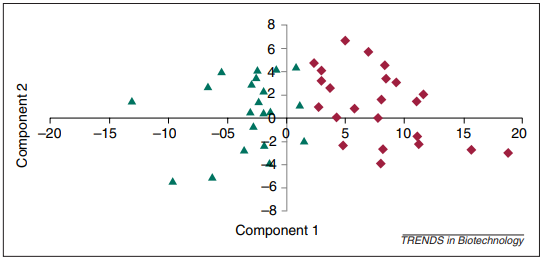
\includegraphics[width=0.7\textwidth]{image.png}
    \caption{Visualization of clustering results for lymphoma subtypes using principal component analysis (PCA). Different shapes indicate distinct subtypes.}
    \label{fig:clustering}
\end{figure}

The clustering results (Figure~\ref{fig:clustering}) show a clear separation of lymphoma subtypes, underscoring the success of the analytical approach. The use of PCA as a dimensionality reduction tool further simplifies the high-dimensional data, enabling intuitive visualization and interpretation of subtype distinctions. Different shapes in the plot correspond to distinct subtypes, indicating that the clustering process effectively captures and represents underlying biological differences.

\section{Conclusion}
Microarray analysis relies on efficient grouping and feature reduction methods to make sense of high-dimensional data. Both supervised and unsupervised techniques play critical roles in extracting biologically meaningful insights. Tools like CLEAVER facilitate these analyses, enabling researchers to focus on key genomic patterns.

\end{document}